\begin{center}
\begin{tikzpicture}[x=1cm,y=1cm]
%\pgfresetboundingbox
\draw[use as bounding box, anchor = north west,draw=none] (-5.5,-3.25) rectangle (5.5,3.25);
\clip (-5.5,-3.25) rectangle (5.5,3.25);
\only<1->{\node[anchor =north west] (text) at (-5.25,3.25){\begin{minipage}{10.0cm}
\scriptsize  Chenru Duan \textit{et. al}. \textit{ChemRxiv} .7616009, ``Learning from Failure: Predicting Electronic Structure Calculation Outcomes with Machine Learning Models", 2019.		
\end{minipage}};}
\visible<1->{\node (figure) at (2.05,1){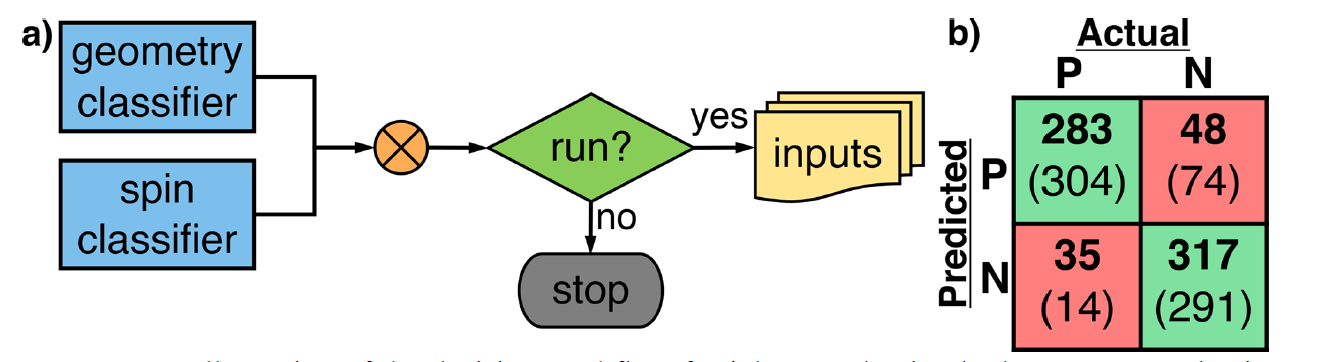
\includegraphics[width=6cm]{applications/images/cd3}};}
\visible<1->{\node (figure) at (2.05,-1.51){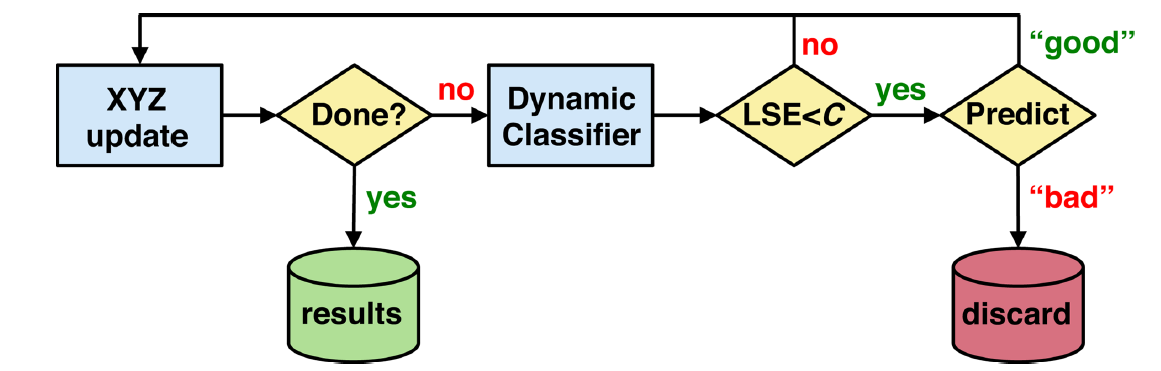
\includegraphics[width=6cm]{applications/images/cd2}};}
\visible<1->{\node[anchor=west] (figure) at (-5.5,0){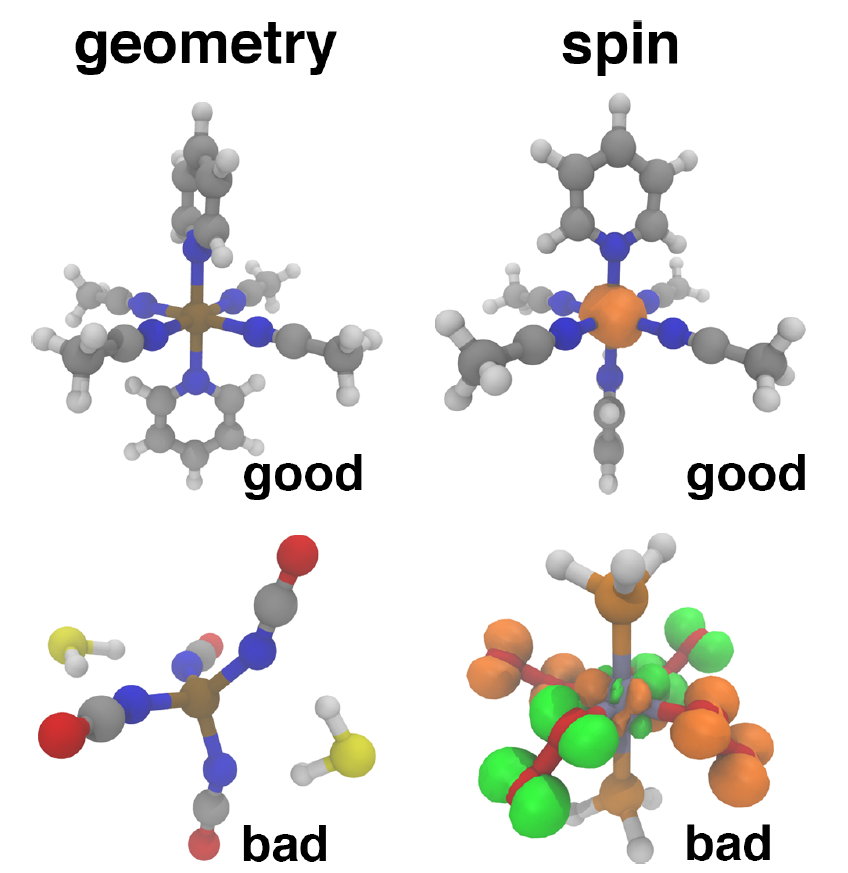
\includegraphics[width=3.5cm]{applications/images/cd1}};}
\end{tikzpicture}
\end{center}